\subsection{Comparison}

In this section we compare the results and methods from \textcite{shitov2020sublinear} and \textcite{kwan2020extension} by working out general similarities and differences. Further, we look at how both bounds are achieved numerically. At the end, we examine how the proofs could be altered to be used in the other's setting.

We start with a quick overview of both results:

\begin{itemize}
  \item \textcite{shitov2020sublinear} proves Theorem~\ref{theorem:xc}, stating that every $n$-gon $P$ has $\xc(P) \in O(n^{2/3})$.
  \item \textcite{kwan2020extension} prove Theorem~\ref{theorem:cyclic-xc}, which states that every cyclic $n$-gon $P$ has $\xc(P) \in O(n^{1/2})$.
\end{itemize}

First we list the general similarities of both approaches:

\begin{itemize}
  \item Both follow the strategy of splitting the polygon into smaller slices.\\
        \citeauthor{shitov2020sublinear} splits the polygon into $12$ slices which are treated separately.\\
        \citeauthor{kwan2020extension} split the polygon into $O(n^{1/2})$ arcs containing $O(n^{1/2})$ vertices, but they are handled interdependently.
  \item There is some notion of enveloping vertices in both.\\
        \citeauthor{shitov2020sublinear} requires an envelope around vertices in the central Theorem~\ref{theorem:gluing}. It is used to build an extended formulation for this specific polygon.\\
        \citeauthor{kwan2020extension} use a ``lampshade argument'', which builds a polygon around vertices away from a set of facets, proving that a part of the slack matrix has constant nonnegative rank.
\end{itemize}

Even though both methods have some ideas in common, they are very different.

\begin{itemize}
  \item \citeauthor{shitov2020sublinear} uses a purely geometric approach.\\
        \citeauthor{kwan2020extension} use the linear-algebraic strategy using slack matrices for their main reasoning. But lemmata are often proved geometrically. The approach has the advantage that transformations on the slack matrix, which don't alter the nonnegative rank, can not always be represented geometrically.
  \item There is another difference in how they treat subsets of vertices:\\
        \citeauthor{shitov2020sublinear} inductively extracts a large subsequence with small extension complexity (ignoring all other vertices).\\
        \citeauthor{kwan2020extension} split their consideration by constantly many colors, but always handle the dependencies to all other vertices.
\end{itemize}

We continue by analyzing how each approach gets to its asymptotical bound numerically.

\citeauthor{shitov2020sublinear}'s result of $\xc(P) \in O(n^{2/3})$ for arbitrary $n$-gons $P$:
\begin{itemize}
  \item There is a subsequence $u$ with $m \in O(n^{2/3})$ vertices for every $n$-gon, for which the main theorem can be applied asymptotically optimal.
  \item It provides the bound $\xc(u) \in O(m^{1/2}) = O(n^{1/3})$ for the extension complexity of that subsequence.
  \item Inductively extracting such a subsequence proves the bound $\xc(P) \in O(n^{2/3})$.
\end{itemize}

\citeauthor{kwan2020extension}'s result of $\xc(P) \in O(n^{1/2})$ for cyclic $n$-gons $P$:
\begin{itemize}
  \item The circle is split into $\abs{\X} \in O(n^{1/2})$ arcs.
  \item The slack matrix is split into $O(1)$ ``color columns'', for which a matrix $K$ with $\rank_+ K \in O(\abs{\X_c})$ is constructed ($\X_c$ are the arcs of color $c$).
  \item Each ``color column'' in the slack matrix has $\rank_+ M[V,F_c] \in O(\abs{\X_c} + n^{1/2})$.
  \item Joining these columns results in $\rank_+ M \in O(\abs{\X} + n^{1/2}) = O(n^{1/2})$.
\end{itemize}

Finally, we have a look at how each procedure could be used in the other's setting:

\begin{itemize}
  \item Even though \citeauthor{kwan2020extension} state that Lemma~10.2 is ``the only place where we use this assumption that $P$ is cyclic'' \cite[22]{kwan2020extension}, the definition of well-separateness uses arc-distance. Generalizing the proof requires something like a boundary-distance, where the distance between two vertices is the sum of the lengths of the edges separating them. In this setting, a counterexample for Lemma~10.2 can be found easily, because well-separated facets and vertices can still have small slacks (see Figure~\ref{fig:cyclic-counter-example}).\\
        We conclude that this approach can't be adopted easily for the general case, since it relies on $P$ being cyclic in central parts. Still, the methods used may be of value for future approaches. This also aligns well with the authors' opinion \cite[28]{kwan2020extension}.
  \item If we want to improve the bound achieved by \citeauthor{shitov2020sublinear} for cyclic polygons, we have to find a larger subsequence for which we can apply Theorem~\ref{theorem:gluing} optimally. In the best case, we can find a subsequence with $\Theta(n)$ vertices, where $\abs{V},\abs{S},\delta \in \Theta(n^{1/2})$ in Theorem~\ref{theorem:gluing}. Then we could obtain the optimal upper bound of $O(n^{1/2})$ for the extension complexity.\\
        Here, we were not able to provide such an improvement.
\end{itemize}

\begin{figure}[ht]
  \centering
  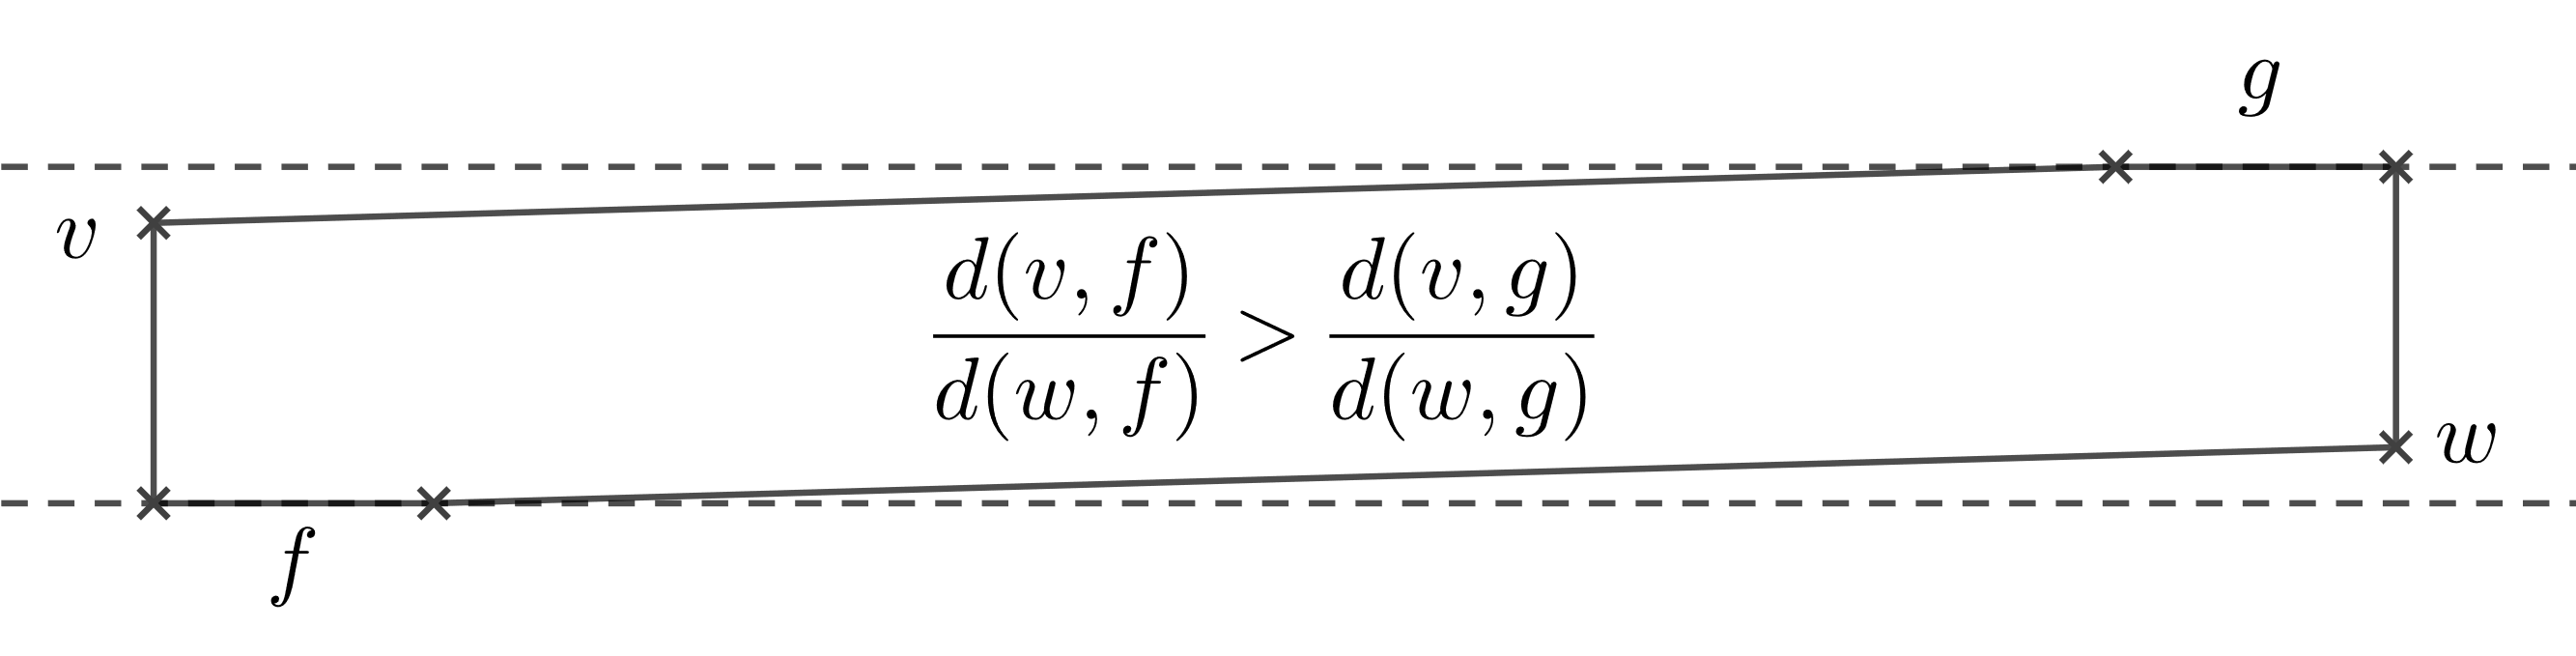
\includegraphics[width=100mm]{cyclic-counter-example.png}
  \caption{Counterexample for Lemma~10.2 \cite{kwan2020extension}, if $P$ weren't cyclic.}
  \label{fig:cyclic-counter-example}
\end{figure}
